\documentclass{beamer}

\usepackage{beamerthemeCVC}

\usepackage{graphicx}

\setbeamertemplate{caption}[numbered]

\usepackage{xmpmulti}

%% PRESENTATION CONFIGURATION PARAMETERS %%%%%%%%%%%%%%%%%%%%%%%%%%%%%%%%%%%%%%%
%  \titlebackgroundfile{images/template_title}
%  \framebackgroundfile{images/template_frame_v05}


%\definecolor{vermell}{HTML}{8C2423}
\definecolor{vermell}{HTML}{000066}
\definecolor{gris}{HTML}{4C4C4C}

% http://latexcolor.com/
\definecolor{anti-flashwhite}{rgb}{0.95, 0.95, 0.96}
\definecolor{palesilver}{rgb}{0.79, 0.75, 0.73}

 
 
\usefonttheme[onlymath]{serif}


%Font 
% \usefonttheme{professionalfonts}
% \usepackage[utf8]{inputenc}
% \usefonttheme{default}


% \usefonttheme[onlymath]{serif}
% % http://tex.stackexchange.com/questions/34265/how-to-get-beamer-math-to-look-like-article-math



% http://tex.stackexchange.com/questions/183052/what-are-all-the-possible-first-arguments-to-setbeamerfont/183053#183053

\setbeamercolor{title in head/foot}{fg=vermell}


\setbeamercolor{author in head/foot}{fg=palesilver}
% 
\setbeamercolor{framenumber in head/foot}{fg=vermell}



\setbeamercolor{section in head/foot}{fg=vermell}
\setbeamercolor{normal text}{fg=gris}
%\setbeamercolor{frametitle}{fg=vermell}
\setbeamercolor{frametitle}{fg=blue!20!black}

\setbeamerfont{block title}{size={}}
\setbeamerfont{author}{size=\footnotesize}
\setbeamerfont{date}{size=\footnotesize}

\setbeamerfont{footline}{size=\fontsize{3}{11}\selectfont}


\setbeamertemplate{itemize item}[circle]
\setbeamertemplate{itemize subitem}[circle]
\setbeamertemplate{itemize subsubitem}[circle]
\setbeamertemplate{itemize subsubsubitem}[circle]
\setbeamercolor{itemize item}{fg=vermell}
\setbeamercolor{itemize subitem}{fg=vermell}
\setbeamercolor{itemize subsubitem}{fg=vermell}
\setbeamercolor{itemize subsubsubitem}{fg=vermell}
\setbeamercolor{enumerate item}{fg=vermell}
\setbeamercolor{enumerate subitem}{fg=vermell}
\setbeamercolor{enumerate subsubitem}{fg=vermell}
\setbeamercolor{enumerate subsubsubitem}{fg=vermell}
\setbeamercolor{alerted text}{fg=vermell}
\setbeamerfont{alerted text}{series=\bfseries}
% This command makes that acrobat reader doesn't changes the colors of the slide
% when there are figures with transparencies.
\pdfpageattr {/Group << /S /Transparency /I true /CS /DeviceRGB>>}



%\setbeamerfont{bibliography entry author}{series=\bfseries}
% \setbeamerfont{bibliography entry title}{series=\bfseries}
% \setbeamerfont{bibliography item}{series=\bfseries}

\setbeamerfont{bibliography item}{size=\scriptsize}
\setbeamerfont{bibliography entry author}{size=\scriptsize}
\setbeamerfont{bibliography entry title}{size=\scriptsize}
\setbeamerfont{bibliography entry location}{size=\scriptsize}
\setbeamerfont{bibliography entry note}{size=\scriptsize}

% \usepackage{hyperref}
% \hypersetup{colorlinks=true, linkcolor=blue}
% \renewcommand*{\bibfont}{\scriptsize}

\graphicspath{{images/}}






%%%%%%%%%%%%%%%%%%%%%%%%%%%%%%%%%%%%%%%%%%%%%%%%%%%%%%%%%%%%%%%%%%%%%%%%%%%%%%%%

%      + Short title.               + Title which appears in the cover.
%      v                            v
%\title[Beamer presentation example]{Nonlinear Dynamics Approach to Human Activity Recognition Using Inertial Sensors}
\vspace{5mm}
\title[Analysis of the Movement Variability in Dance Activities Using Wearable Sensors]
{Analysis of the Movement Variability in Dance Activities Using Wearable Sensors}
%       + Short author names which appear in the slides.
%       v
\author[Miguel P. Xochicale]
{   % Author names which appear in the cover page.
    %Perez-Xochicale Miguel Angel
    Miguel P. Xochicale\inst{1}, Chris Baber\inst{1} and Mourad Oussalah\inst{2}
}
%          + Short affiliation which appears in the slides.
%          v
\institute[CVC-IIIA]
{   % Affiliation information which appears in the cover page.

      \vspace{5mm}
    \begin{tabular}{c}
    \inst{1} School of Electronic, Electrical and System Engineering, University of Birmingham, U.K. \\
    \inst{2} Center for Ubiquitous Computing, University of Oulu, Finland
    \end{tabular}
}
%     + Short acronym of the conference or date of the presentation.
%     v
\date[DEMO-2013]
{   % Conference name which appears in the cover page.
      \vspace{5mm}
     The 2nd International Symposium on Wearable Robotics \\
     La Granja de San Idelfonso, Segovia, Spain \\
     18-21 October 2016
}


% 
% \AtBeginSection[]{
%   \begin{frame}
%   \vfill
%   \centering
%   \begin{beamercolorbox}[sep=8pt,center,shadow=true,rounded=true]{title}
%     \usebeamerfont{title}\insertsectionhead\par%
%   \end{beamercolorbox}
%   \vfill
%   \end{frame}
% }


\AtBeginSubsection[]
{
   \begin{frame}
        \frametitle{Outline}
        \tableofcontents[currentsection,currentsubsection]
   \end{frame}
}






\begin{document}
% Creates the cover page.
\frame{\titlepage}





\begin{frame}
\frametitle{Outline} 
\tableofcontents
\end{frame}




%+++++++++++++++++++++++++++++++++++++++++++++++++++
%+++++++++++++++++++++++++++++++++++++++++++++++++++
\section{I. Introduction: Movement Variabily}

% %+++++++++++++++++++++++++++++++++++++++++++++++++++
\begin{frame}
  \frametitle{Why Movement Variablity in Dance?}

  
  \begin{figure}
 \includegraphics[width=0.7\textwidth]{hri_tmr2013_01}
\centering 
\caption{Dance Demo with a Robot at the Mexican Robotics Tournament 2013}
 \end{figure}
 
 
\end{frame}




 
 
 
%%+++++++++++++++++++++++++++++++++++++++++++++++++++
\begin{frame}
\frametitle{Movement Variability}
 
Movement Variability is an inherent feature that occurs not only across but within individuals
and across systems of movement  \textcolor{red}{\textbf{ \cite{newell1993variability}   }}.
  
\end{frame}
 
%%+++++++++++++++++++++++++++++++++++++++++++++++++++
\begin{frame}
\frametitle{Inter-trial Movement Variability}
 
Inter-trial variability ($V_{tot}$) is a combination of noise ($V_{e}$) in 
% the neuro-musculo-skeletal system :
\begin{itemize}
    \item sensory information and motor output commands ($V_{eb}$)
    \item changes in the enviromental conditions ($V_{ee}$)
    \item measuring and data processing techniques ($V_{em}$)
\end{itemize}
and functional changes that might be associated with the exploration of different 
stragies to find the most effective one among many available ($V_{nl}$) 
\textcolor{red}{\textbf{  \cite{Preatoni2013}   }}.

\begin{eqnarray*} 
 V_{tot} = V_{e} + V_{nl}
\end{eqnarray*}


\end{frame}
 
 
 
  
 
 
 % %+++++++++++++++++++++++++++++++++++++++++++++++++++
\begin{frame}
  \frametitle{Motor Variability is not noise}

  
  \begin{figure}
 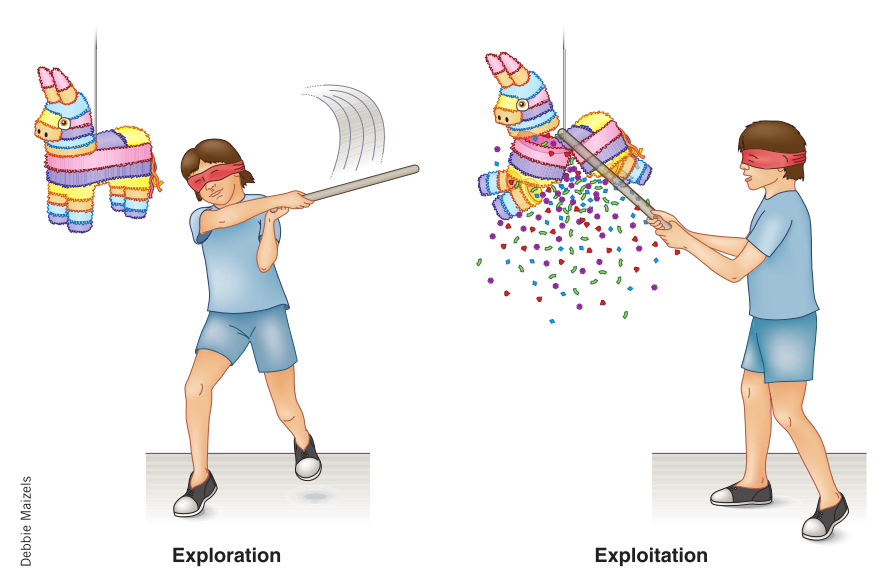
\includegraphics[width=0.7\textwidth]{herzfelt2014_fig1}
\centering 
\caption{Find the pi\~nata \textcolor{red}{\textbf{  \cite{Herzfeld2014}   }}.}
 \end{figure}
 
 

 
 
\end{frame}




 
%%+++++++++++++++++++++++++++++++++++++++++++++++++++
\begin{frame}
\frametitle{Nonlinear Dynamics to  Movement Variability}
 

According to \textcolor{red}{\textbf{  \cite{Preatoni2013}   }},
some nonlinear dynamics tools to explore the nature of movement variability 
and its relationship with skills development are:
\begin{itemize}
    \item Phase Space Representation
    \item Lyapunov Exponent.
\end{itemize}


\end{frame}
 
 


%+++++++++++++++++++++++++++++++++++++++++++++++++++
%+++++++++++++++++++++++++++++++++++++++++++++++++++
\section{II. Methods}

 
 \subsection{Activity Recognition Chain}
 

%+++++++++++++++++++++++++++++++++++++++++++++++++++
\begin{frame}
\frametitle{Activity Recognition Chain for Inertial Sensors}
\vspace{-0.7cm}


\begin{figure}[!htb]
\centering    
\includegraphics[width=0.85\textwidth]{banos2014_ARC_3}
\caption[PA]{Window Size impact in ARC
 \textcolor{red}{\textbf{ \cite{Banos2014} }}.
}  
\label{fig:sn}
\end{figure}



\end{frame}
%---------------------------------------------------



%+++++++++++++++++++++++++++++++++++++++++++++++++++
\begin{frame}
  \frametitle{Feature extraction Using Inertial Sensors}

\begin{figure}[!htb]
\centering    
\includegraphics[width=1\textwidth]{figo_2010_feature_extraction_v04}
\caption[PA]{Techniques applied to accelerometer sensor signals for feature extraction 
\textcolor{red}{\textbf{ \cite{Figo2010,Liao2015,Gupta2014,Fish2012,Zhang2011} }}.
}  
\label{fig:sn}
\end{figure}

\end{frame}
%---------------------------------------------------





\subsection{Time-delay embedding}








%+++++++++++++++++++++++++++++++++++++++++++++++++++
\begin{frame}
\frametitle{Time-delay embedding theorem}


For a given discrete time-series $x(n) = [x(1) , x(2), \dots, x(N)]$,
a reconstructed state space can be created by
\begin{eqnarray*} 
\overline{x}(n) = [ x(n), x(n - \tau), x(n-2\tau), \dots , x (n-(m-1)\tau) ]
\end{eqnarray*}
which creates a concatenated column-wise matrix of the time-delay versions of the original signal:
\begin{equation}
  \resizebox{\textwidth}{!}{$\displaystyle
  \mathbf{X}
    = \begin{pmatrix} \nonumber
      x(1) & x(1 - \tau) & x(1-2\tau) & \dots & x (1-(m-1)\tau) \\
      x(2) & x(2 - \tau) & x(2-2\tau) & \dots & x (2-(m-1)\tau) \\
      \vdots &  &  & \ddots & \vdots \\
      x(N) & x(N - \tau) & x(N-2\tau) & \dots & x (N-(m-1)\tau) \\
      \end{pmatrix}
     $}
\end{equation}
        
        

where $m$ is the \textbf{ embedding dimension}  and  $\tau$ is the \textbf{ embedding delay}
\textcolor{red}{\textbf{  \cite{Takens1981} }}.



% of the original system is given by 
% %the delay coordinate (DC) vector

%  
% The time-delay embeddings method, states
% that for a large enough $m$ to unfold the attractor and $\tau > 0$ 
% chosen to maximize the information content of $x(t)$, this method provides a 
% one-to-one reconstruction of the true dimension $k$ system ($\mathbb{R}^k$).

\end{frame}
%---------------------------------------------------




%+++++++++++++++++++++++++++++++++++++++++++++++++++
\begin{frame}
\frametitle{Time-delay embedding theorem}

The time-delay embeddings theorem states that for a large enough $m$ is possible to unfold the attractor 
and $\tau > 0$ is chosen to maximize the information content of $x(n)$.

False Nearest Neighborhood and Mutual Information algorithms are used to compute
the optimal value of $m$ and $\tau$. However, as pointed out by  \textcolor{red}{\textbf{ \cite{Sama2013} }}
the optimal values don't neccesarily represent the best rate of recognition.
% which means that
% the embedded values are dependant of the activity to recognise.



\end{frame}
%---------------------------------------------------






%+++++++++++++++++++++++++++++++++++++++++++++++++++
\begin{frame}
\frametitle{Principal Component Analysis (PCA)}
\vspace{-0.7cm}

The Percentage of Cumulative Energy (PCE) is obtained by using the PCA \textcolor{red}{\textbf{ \cite{Hammerla2011} }}.
For each eigenvalue $\lambda_i$, the cummulative energy is
\begin{eqnarray*} 
C_i = \frac{ \Sigma_{j=1}^{i} \lambda_j }{ \Sigma_{k=1}^{m} \lambda_k }
\end{eqnarray*}
then, the area under the curve is computed to obtain the PCE.


\begin{figure}[!htb]
\centering    
\includegraphics[width=1\textwidth]{method_diagram02}
\caption[PA]{Percentage of Cummulative Energy}
 \label{fig:sn}
\end{figure}


\end{frame}
%---------------------------------------------------




%+++++++++++++++++++++++++++++++++++++++++++++++++++
\begin{frame}
\frametitle{Time-delay embedding}
\vspace{-0.7cm}


\begin{figure}[!htb]
\centering    
\includegraphics[width=1\textwidth]{frank_2012}
\caption[PA]{3-D Reconstructed State Spaces for walking (left), running (middle), and cycling (right) $m=3$, $\tau=4$ . 
 \textcolor{red}{\textbf{ \cite{Frank2010,Frank2012} }}.
}  
\label{fig:sn}
\end{figure}

\end{frame}
%---------------------------------------------------


%+++++++++++++++++++++++++++++++++++++++++++++++++++
\begin{frame}
\frametitle{Time-delay embedding}
\vspace{-0.7cm}



\begin{figure}[!htb]
\centering    
\includegraphics[width=0.6\textwidth]{sama_2013}
\caption[PA]{2-D Reconstructed State Spaces for gait patterns of two persons ($m=20$ for $\tau=1$, $\tau=4$ and $\tau=9$, respectively). 
 \textcolor{red}{\textbf{ \cite{Sama2013} }}.
}  
\label{fig:sn}
\end{figure}



\end{frame}
%---------------------------------------------------










%+++++++++++++++++++++++++++++++++++++++++++++++++++
\begin{frame}
\frametitle{[Time-delay embedding for Emotion Recognition ] }
\vspace{-0.7cm}


\begin{figure}[!htb]
\centering    
\includegraphics[width=1\textwidth]{emotionrecognition00}
\caption[PA]{Time delay embeddings for two male and two female
expresing sentences of anger and joy ($m=3$ for $\tau=1$) \textcolor{red}{\textbf{  \cite{Harimi2015} }}. }
  
\label{fig:sn}
\end{figure}



\end{frame}
%---------------------------------------------------



% 
%  
%   % %+++++++++++++++++++++++++++++++++++++++++++++++++++
% \begin{frame}
%   \frametitle{Movement Variability}
%   
%  2. Measuring human movements using inertial sensors
% 3. Methodologies (Time-series Features)
%    3.2 Time-domain features
%    3.3 Frequency-domain features
%    3.4 Non-linear dynamics
%       3.4.1. Time-delay embedding (Taken's Theorem)
% 4. Pilot Experiment (Salsa Dance)
% 5. Outcome
% 6. Work in Progress
% 7. Conclusions
%  
% 
%  
%  \end{frame}
%  

 
 

%+++++++++++++++++++++++++++++++++++++++++++++++++++
%+++++++++++++++++++++++++++++++++++++++++++++++++++
\section{III. Experiment}
 
\subsection{Design}
 
 

 

%+++++++++++++++++++++++++++++++++++++++++++++++++++
\begin{frame}
\frametitle{Basic Salsa Steps}
\vspace{-0.7cm}


\begin{figure}[!htb]
\centering    
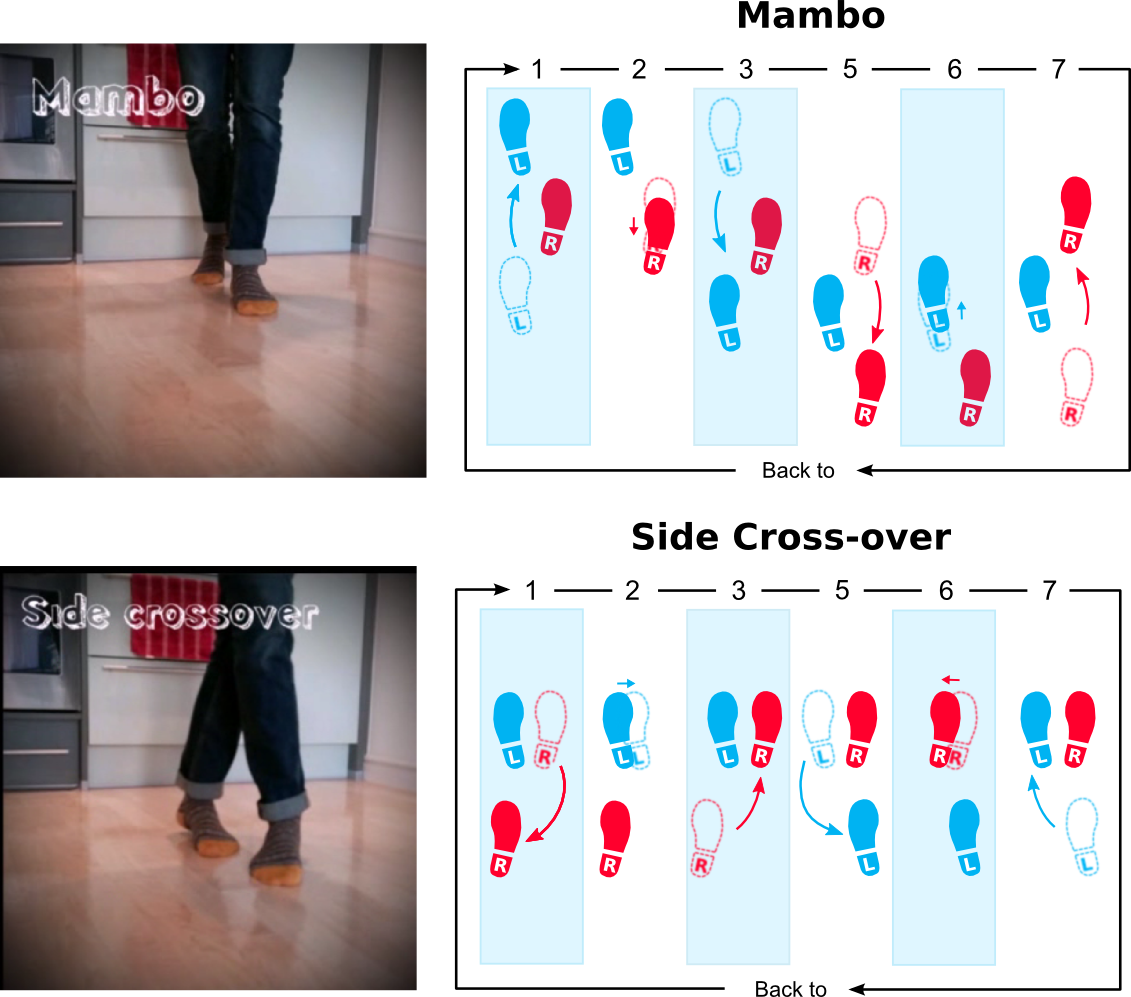
\includegraphics[width=0.7\textwidth]{steps00}
\caption[PA]{}
  
\label{fig:sn}
\end{figure}



\end{frame}
%---------------------------------------------------



\subsection{Results}




 

%+++++++++++++++++++++++++++++++++++++++++++++++++++
\begin{frame}
\frametitle{Dancers time-series}
\vspace{-0.7cm}


\begin{figure}[!htb]
\centering    
\includegraphics[width=1\textwidth]{timeseries00}
\caption[PA]{}
  
\label{fig:sn}
\end{figure}



\end{frame}
%---------------------------------------------------



 
 

 

%+++++++++++++++++++++++++++++++++++++++++++++++++++
\begin{frame}
\frametitle{2-D R}
\vspace{-0.7cm}


\begin{figure}[!htb]
\centering    
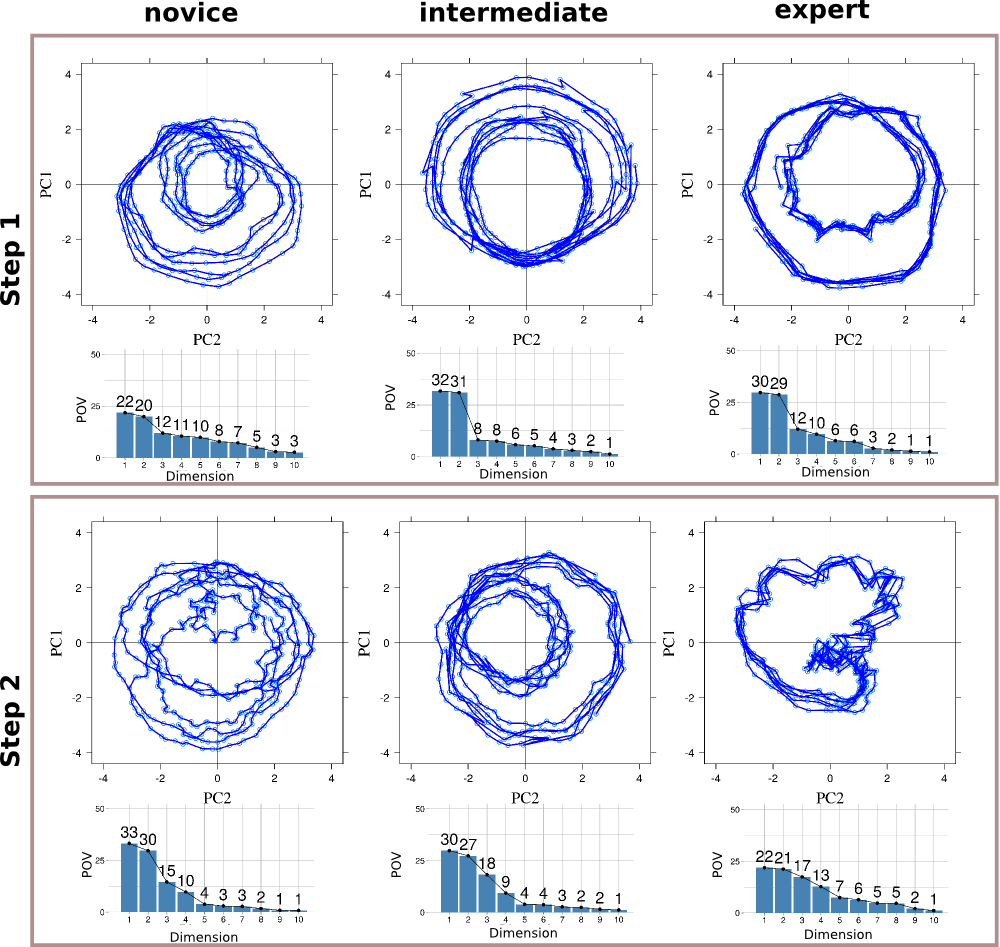
\includegraphics[width=0.7\textwidth]{main_figure_horizontal02}
\caption[PA]{}
  
\label{fig:sn}
\end{figure}



\end{frame}
%---------------------------------------------------





  
%+++++++++++++++++++++++++++++++++++++++++++++++++++
%+++++++++++++++++++++++++++++++++++++++++++++++++++
\section{Conclusions and Future Work}


%+++++++++++++++++++++++++++++++++++++++++++++++++++
\begin{frame}
\frametitle{Segmentation Analysis}
\vspace{-0.7cm}


\begin{figure}[!htb]
\centering    
\includegraphics[width=.7\textwidth]{statistics00}
\caption[PA]{}
  
\label{fig:sn}
\end{figure}



\end{frame}
%---------------------------------------------------



 
%+++++++++++++++++++++++++++++++++++++++++++++++++++
\begin{frame}
\frametitle{Novice Dancers time-series}
\vspace{-0.7cm}


\begin{figure}[!htb]
\centering    
\includegraphics[width=1\textwidth]{novice_timeseries00}
\caption[PA]{}
  
\label{fig:sn}
\end{figure}



\end{frame}
%---------------------------------------------------


 
%+++++++++++++++++++++++++++++++++++++++++++++++++++
\begin{frame}
\frametitle{Future Work}
\vspace{-0.7cm}


\begin{figure}[!htb]
\centering    
\includegraphics[width=0.7\textwidth]{fw00}
\caption[PA]{Testing variability across participants  }
  
\label{fig:sn}
\end{figure}



\end{frame}
%---------------------------------------------------



 
 
 
%  
%  
% 
% %+++++++++++++++++++++++++++++++++++++++++++++++++++
% \begin{frame}
% \frametitle{PhD Framework for February and March}
% \vspace{-0.7cm}
% 
% \textbf{FEBRUARY}
%     \begin{itemize}
%     \item Create Artificial Structure Signals.
%     \item Apply Statistical and Nonlinear methods to analise the variability of artificial signals.
%     \item Pilot Data Collection Experiment Using Commertial and non-commertial IMUs.
%     \end{itemize}
% \textbf{MARCH}    
%     \begin{itemize}
%     \item Pilot classification experiment with SVM or a technique of deep learning \\ (collaboration with \textit{Dr. Mourad Oussalah})
%     \item Submit the advances to the International Symposium on Wearable Computers (ISWC) 2016 (Deadline ist April 16, 2016)
%     \end{itemize}    
%     
% %    Deep Convolutional and LSTM Recurrent Neural Networks for Multimodal Wearable Activity Recognition.
% %Ordóñez FJ1, Roggen D2.
% 
% \end{frame}
% %---------------------------------------------------




%   \section[allowframebreaks]{References}
 
%  \section{V. Conclusions and Future Work}


 \begin{frame}[fragile,allowframebreaks]{References}
  % In your presentation, remove `\nocite` here and
  % use `\cite` throughout the presentation.
  \nocite{*}
  
  \bibliographystyle{apalike}
  \bibliography{refslides}


%  \bibliography{D:/Gpai/Biblographies/library}
\end{frame}





%+++++++++++++++++++++++++++++++++++++++++++++++++++
\begin{frame}
\frametitle{}

\vspace{2cm}
\begin{center}
\LARGE{QUESTIONS?} 
\end{center}

\vspace{1cm}

\normalsize 
\textbf{Miguel Xochicale} \\
Doctoral Researcher in Human-Robot Interaction \\
University of Birmingham, U.K. \\ 
{\color{blue} \href{http://mxochicale.github.io/}{http://mxochicale.github.io/ } } \\

   
\vspace{1cm}



\includegraphics[scale=.4]{CC4}
\tiny{ 
\textbf{My own pictures are release under CC BY-NC 4.0
{\color{blue} \href{http://creativecommons.org/licenses/by-nc/4.0/}{http://creativecommons.org/licenses/by-nc/4.0/} } \\
Give credits to: Miguel Xochicale
}
}

\end{frame}
%---------------------------------------------------

% 
% % Creates the cover page.
%  \frame{\titlepage}



\end{document}

